% !TeX root = ../thuthesis-example.tex

\chapter{Introduction}

Enzymes are proteins that catalyze biological reactions. They accelerate reactions 
to a speed that supports metabolic processes necessary for life. 
Understanding how enzymes work is crucial not only for grasping fundamental 
biological mechanisms but also for advancing medical science, 
particularly in the development of new pharmaceuticals and the engineering 
of enzymes with enhanced properties.

In order to design effective drugs or improve enzyme functions, 
one major challenge is the selection of the most promising compounds 
from a vast array of possibilities. 
Laboratory testing is costly and time-consuming. To reduce the possibilities,
using kinetic information can become a promising solution.

A key parameter in enzyme kinetics is the Michaelis constant ($K_m$). It represents
the substrate concentration at which the initial velocity of the reaction is half of
the maximum velocity. Generally, the lower the value, the higher is the affinity 
between the enzyme and the substrate.

Predicting the Michaelis constant can significantly accelerate the drug design process. 
By estimating an enzyme's affinity for various substrates and similarly, several enzymes
with one substrate, researchers can prioritize compounds for further development, 
thereby reducing the need for extensive laboratory testing. 
This approach not only facilitates the discovery of new drugs but also enhances 
our ability to engineer enzymes with desired characteristics.

\section{Problem statement}

The goal of this work is to build a statistical regression model that predict the 
Michaelis constant given on 2 inputs: the protein sequence and the substrate string. 

The performance of the model will be evaluated with the mean squared error (MSE) and 
the coefficient of determination $r^2$.

\section{Literature review}

Given the interdisciplinary nature of this thesis, which involves biological, chemical, and 
computer sciences, the literature review will be structured in the following way.

First, the reader will be provided with the biological and chemical fundamentals necesarry to understand basic aspects
of enzyme kinetics. This foundation is essential to comprehend the biological processes at play and
their relevance to our work.

Second, machine learning and deep learning methodologies, emphasizing on their biological
applications, will be presented. This section aims to present how statistical models can be used to decipher complex biological
data, hence allowing us to build innovative solutions in enzyme and drug design.

Finally, a specific focus on the current state of research regarding the prediction of the Michaelis 
constant ($K_m$) will be provided. This aim of this part is there to highlight the current contributions to 
our problem statement, the current state-of-the-art methods used, and their results.

Through this comprehensive review,the solid background provided will ensure the relevance of this thesis
contribution in the field of drug design. 

\subsection{Biological and Chemistry Background}
\subsubsection{Proteins}
Proteins impact all the processes that take place in a cell, with an almost
endless diversity of functions. They are the most abundant biological macromolecules.
Thousands of different types of proteins can be found in a single cell. They are the molecular
instruments through which genetic information is expressed.\cite{lehninger}.

A protein is a sequence of smaller molecules called amino acids that are covalently joined by a peptide
bond. There exists 20 common amino acids (Figure \ref{fig:20aa}) from which almost all proteins are made of. Each amino acid has
a side chain with distinctive chemical properties.

\begin{figure}
  \centering
  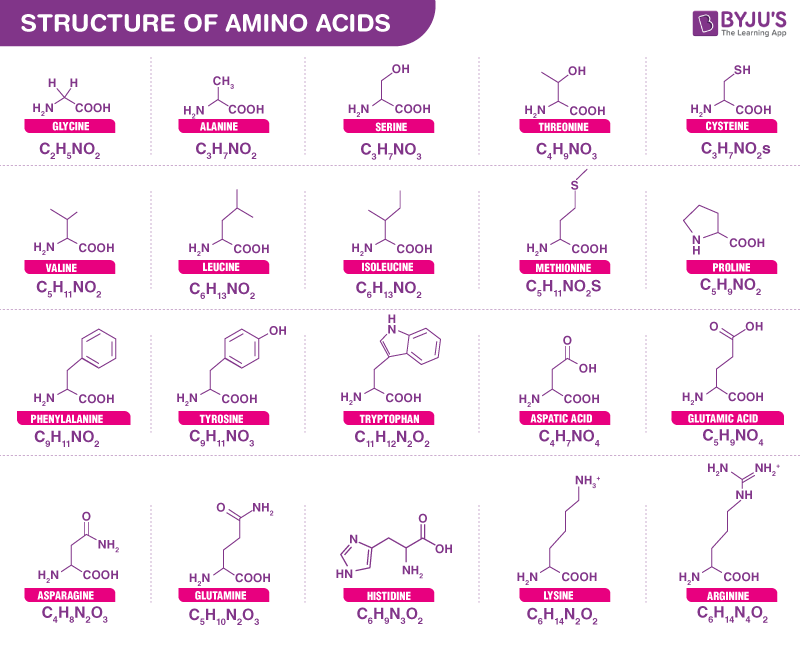
\includegraphics[width=0.7\linewidth]{1-amino_acids.png}
  \caption{The 20 common amino acids}
  % https://www.google.com.hk/url?sa=i&url=https%3A%2F%2Fbyjus.com%2Fbiology%2Famino-acids%2F&psig=AOvVaw1r9URV_-jl8bxr1TZ5ehjk&ust=1710296952635000&source=images&cd=vfe&opi=89978449&ved=0CBMQjRxqFwoTCIjpnuXW7YQDFQAAAAAdAAAAABAE
  \label{fig:20aa}
\end{figure}

All common amino acids are $\alpha$-amino acids. This means that both the carboxyl group and the amino group
is bonded to the same carbon atom called the $\alpha$-carbon (Figure \ref{fig:aastructure}). The amino acids differ from each others in
their side chains, also called R-groups, which vary in size, structure, electronic charge, and which
influence the solubility of the amino acids in water.

\begin{figure}
  \centering
  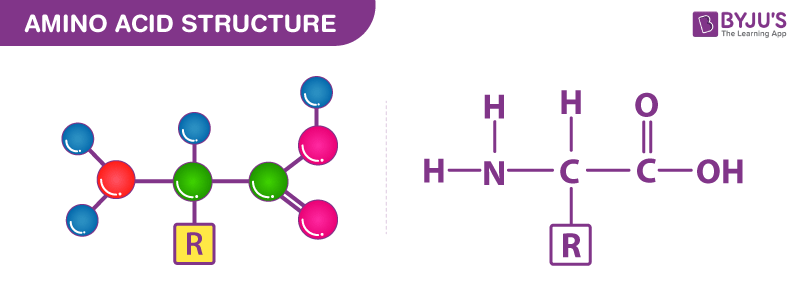
\includegraphics[width=0.3\linewidth]{1-amino_acid_structure.png}
  \caption{Amino acid structure}
  % https://www.google.com.hk/url?sa=i&url=https%3A%2F%2Fen.wikipedia.org%2Fwiki%2FAmino_acid&psig=AOvVaw1uUyMqtMb_u6DnLzN1XZTr&ust=1710297308181000&source=images&cd=vfe&opi=89978449&ved=0CBMQjRxqFwoTCOiroY7Y7YQDFQAAAAAdAAAAABAD
  \label{fig:aastructure}
\end{figure}

Two amino acids can be joined together with a covalent bond that is called a peptide bond. This link
is formed by the removal of the element of water (a hydroxyl group from the $\alpha$-carboxyl group
of one amino acid and a hydrogen atom from the $\alpha$-amino group of another amino acid. Figure 
\ref{fig:peptidebond}). These joined amino acids are called residues, relfecting the loss of the element
of water during the bonding formation.

\begin{figure}
  \centering
  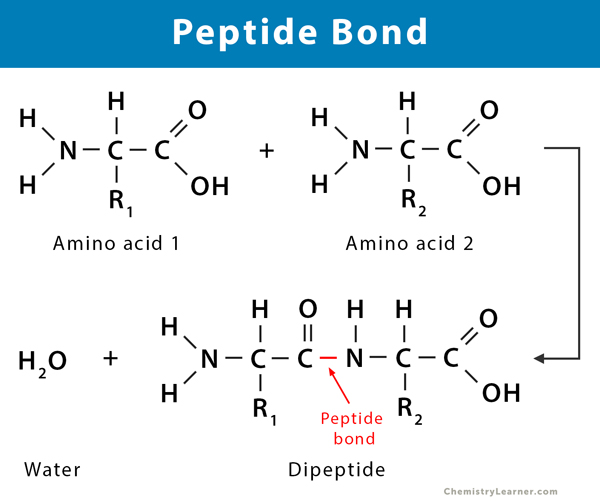
\includegraphics[width=0.5\linewidth]{1-peptide_bond.jpeg}
  \caption{Peptide bond}
  %https://www.chemistrylearner.com/wp-content/uploads/2020/10/Peptide-Bond.jpg
  \label{fig:peptidebond}
\end{figure}

An oligopeptide is the structure of a few amino acids joined together and a polypeptide is the name
given to the structure when many amino acids are joined. Proteins may have thousands of amino acids residues.

For proteins, the amino acid residues at the end are the $\alpha$-amino group called N-terminal and 
the $\alpha$-carboxyl group called C-terminal. The N-terminal is conventionally placed on the left while
the C-terminal is placed on the right.

The functions of proteins do not depend on their length or molecular weight. Some very small proteins 
(2 to 10 amino acids) can be extremely important such as toxic mushroom poisons or antibiotics (example + ref). The
length of proteins can vary enourmously from 2 to 27,000 amino acids, while the vast majority of proteins
usually contain fewer than 2,000 amino acids.

Some proteins are made of only one polypeptide chain while other can be made out of several, they are 
called mutlisubunit proteins, such as hemoglobin (example + ref).

Some proteins also contain chemical groups other than amino acids. They are called conjugated proteins.
The non-amino acid part of these proteins is called its prosthetic group and is essential to the protein
overall functions, such as hemoglobin and its ferrous group without which it does not function properly 
(check this + example + ref)

\subsubsection{Enzymes}
Enzymes are specific proteins that accelerate the rate of reactions. They are essential to life as many
of the chemical reactions essential to our survival need to be accelerated, such as the conversion of sugar.
(add example). 

xxx
\subsubsection{Substrates}
Substrates are the small molecules that interact with enzymes.

xxx
\subsubsection{Enzyme Kinetics}
kcat and Km

\subsection{Machine and Deep Learning for Drug Discovery}
\subsubsection{Traditional approaches}
\subsubsection{Machine Learning approaches}
\subsubsection{Neural Networks}
\subsubsection{Protein Language Models}
\subsubsection{Graph Neural Networks}

\subsection{Michaelis constant prediction}
\subsubsection{Current methods}
\subsubsection{State-of-the-art model performances}

\section{Methodology}
This research will be composed of a data preprocessing step, a model implementation step, and an
evaluation step.
\subsection{Data preprocessing}
In this work, we will use a dataset curated by (Prosmith), using data from BRENDA (ref) which is a
xxxxxx (explainantion of the database).
The data used is up to 2022. Therefore, we will augment their dataset with a new test set composed of
the data from 2022 to January 2024, allowing a better testing of the current methods and the validation
of this work.
The data will be processed in a way to obtain 3 elements: the protein sequence, the substrate string,
and the Michaelis constant value.
\subsection{Model implementation}
The model implementation will be composed of 3 parts. The first one will be the creation of an architecture
for the sequence-based model, the for the structure-based model, and finally for the ensemble model using both
the sequence-based and the structure-based model.
\subsection{Model evaluation}
The 3 models of this work (sequence-based model, structure-based model, and sequence-structure-based model)
will be evaluated on the ProSmith test set as well as our newly curated test set. The evaluation metrics 
wil be the mean squared error (MSE) and the coefficient of determination $r^2$.

Not only will this work evaluate these metrics in the general sense but it will also provide a more specific
set of these metrics based on the data: the protein sequences and the substrates strings will be divided into
4 groups based on their appearance in the training set. Proteins that have been seen in the training set
will be denoted "hot proteins" and the ones that are not in the training set "cold proteins". Similarly, 
subrates included in the training set will be denoted "hot substrates" and "cold substrates" if they
are not.

These 4 groups will allow a better comparison of this work method and the state-of-the-art methods.

